% Presentación de la defensa — Proyecto final de Cálculo Multivariable (UCC 2026B)
% Compilar desde esta carpeta:  pdflatex defensa.tex && pdflatex defensa.tex
% Notas del orador: están en \note{...}. Para verlas, descomentar la línea de pgfpages.
\documentclass[aspectratio=169,11pt]{beamer}

\usepackage[spanish,es-nodecimaldot]{babel}
\usepackage[T1]{fontenc}
\usepackage{lmodern}
\usepackage{amsmath,amssymb,bm}
\usepackage{booktabs,array,tabularx}
\usepackage{graphicx}
\usepackage{tikz}
\graphicspath{{../graficos/}}
% \usepackage{pgfpages}\setbeameroption{show notes on second screen=right}

% ---------- Estilo ----------
\definecolor{tinta}{HTML}{10182B}
\definecolor{papel}{HTML}{F6F3EC}
\definecolor{arena}{HTML}{ECE6D9}
\definecolor{cuerpo}{HTML}{3B4456}
\definecolor{acento}{HTML}{C4561F}
\definecolor{naranja}{HTML}{E0703A}

\usetheme{default}
\setbeamercolor{background canvas}{bg=papel}
\setbeamercolor{normal text}{fg=cuerpo}
\setbeamercolor{frametitle}{fg=tinta}
\setbeamercolor{framesubtitle}{fg=acento}
\setbeamercolor{structure}{fg=acento}
\setbeamercolor{block title}{fg=acento,bg=arena}
\setbeamercolor{block body}{fg=cuerpo,bg=arena}
\setbeamerfont{frametitle}{size=\Large,series=\bfseries}
\setbeamerfont{framesubtitle}{size=\scriptsize,series=\bfseries}
\setbeamerfont{block title}{size=\scriptsize,series=\bfseries}
\setbeamertemplate{navigation symbols}{}
\setbeamertemplate{blocks}[rounded]
\setbeamertemplate{itemize items}{\color{naranja}\textbullet}
\setbeamertemplate{frametitle}{%
  \vspace*{0.6em}%
  {\usebeamerfont{framesubtitle}\usebeamercolor[fg]{framesubtitle}\MakeUppercase{\insertframesubtitle}\par}%
  \vspace{0.15em}%
  {\usebeamerfont{frametitle}\usebeamercolor[fg]{frametitle}\insertframetitle\par}%
  \vspace{0.2em}}
\setbeamertemplate{footline}{%
  \hfill{\scriptsize\usebeamercolor[fg]{normal text}\insertframenumber\,/\,\inserttotalframenumber}\hspace*{1.2em}\vspace*{0.8em}}

% Tarjeta: \tarjeta{TÍTULO}{texto}; con paso de aparición: \tarjeta[<2->]{TÍTULO}{texto}
\newcommand{\tarjeta}[3][]{%
  \begin{block}#1{\MakeUppercase{#2}}\small #3\end{block}}
% Lo que aún no aparece no se ve, pero conserva su espacio (la diapositiva no salta)
\setbeamercovered{invisible}
% Diapositiva oscura / de acento
\newenvironment{oscura}{\setbeamercolor{background canvas}{bg=tinta}\setbeamercolor{normal text}{fg=papel}\setbeamercolor{frametitle}{fg=papel}\setbeamercolor{framesubtitle}{fg=naranja}\setbeamercolor{block body}{fg=papel,bg=tinta!80!white}\setbeamercolor{block title}{fg=naranja,bg=tinta!80!white}\usebeamercolor[fg]{normal text}}{}
\newenvironment{acento}{\setbeamercolor{background canvas}{bg=naranja}\setbeamercolor{normal text}{fg=tinta}\setbeamercolor{frametitle}{fg=tinta}\setbeamercolor{framesubtitle}{fg=tinta}\setbeamercolor{block body}{fg=tinta,bg=naranja!55!white}\setbeamercolor{block title}{fg=tinta,bg=naranja!55!white}\usebeamercolor[fg]{normal text}}{}

\newcommand{\grande}[1]{{\fontsize{30}{32}\selectfont\bfseries\color{tinta}#1}}

\title{La ley de Hubble como problema de optimización}
\subtitle{Regresión lineal $y = ax + b$ que minimiza $S(a,b) = \sum (y_i - a x_i - b)^2$}
\author{Juan Camilo López Díaz \\ Jenifer Daniela Urbano Córdoba \\ Nicolás Alejandro Díaz Acosta \\ José Nicolás Mora Delgado \\ Drako David Salazar Torres}
\institute{Universidad Cooperativa de Colombia · Cálculo Multivariable · 2026B\\Docente: M.Sc. Alejandro Molina}
\date{}

\begin{document}

% =====================================================================
% 1. PLANTEAMIENTO
% =====================================================================
{\begin{oscura}
\begin{frame}[plain]
  \begin{columns}[c]
    \begin{column}{0.55\textwidth}
      {\scriptsize\bfseries\color{naranja}PROYECTO FINAL · CÁLCULO MULTIVARIABLE}\par\vspace{0.8em}
      {\LARGE\bfseries\color{papel}\inserttitle\par}\vspace{0.8em}
      {\small\insertsubtitle\par}\vspace{1.4em}
      {\scriptsize\insertinstitute\par\vspace{0.8em}
       {\bfseries\color{naranja}INTEGRANTES}\par\vspace{0.2em}\insertauthor\par}
    \end{column}
    \begin{column}{0.42\textwidth}
      % Los 24 datos reales de Hubble y la recta de ajuste (motivo decorativo)
      \begin{tikzpicture}[x=2.6cm,y=0.0026cm]
        \foreach \x/\y in {0.032/170,0.034/290,0.214/-130,0.263/-70,0.275/-185,0.275/-220,0.45/200,0.5/290,0.5/270,0.63/200,0.8/300,0.9/-30,0.9/650,0.9/150,0.9/500,1.0/920,1.1/450,1.1/500,1.4/500,1.7/960,2.0/500,2.0/850,2.0/800,2.0/1090}
          \fill[papel,opacity=0.85] (\x,\y) circle (2.2pt);
        \draw[naranja,line width=2pt,line cap=round] (0,-40.78) -- (2.1,{454.16*2.1-40.78});
      \end{tikzpicture}
    \end{column}
  \end{columns}
  \note{Presentar al grupo y el tema. El dibujo son los 24 datos reales de Hubble con la recta que vamos a obtener: toda la exposición explica cómo se llega a esa recta con Cálculo Multivariable.}
\end{frame}
\end{oscura}}

{\begin{acento}
\begin{frame}{¿Cómo se puede utilizar el Cálculo Multivariable para determinar y analizar el modelo lineal que mejor representa un conjunto de datos?}
  \framesubtitle{Pregunta central}
  \vfill
  \begin{columns}[T]
    \column{0.31\textwidth}\tarjeta[<2->]{Analítica}{Derivadas parciales, $\nabla S = \mathbf{0}$ y Hessiano, hechos a mano.}
    \column{0.31\textwidth}\tarjeta[<3->]{Geométrica}{Superficie de error, trazas y curvas de nivel.}
    \column{0.31\textwidth}\tarjeta[<4->]{Computacional}{Código propio que verifica y visualiza, no que reemplaza.}
  \end{columns}
  \note{Es la pregunta del enunciado. La respondemos desde tres miradas: primero el cálculo a mano, luego la geometría de la función de error y por último el computador como verificación.}
\end{frame}
\end{acento}}

\begin{frame}{Hubble, 1929: cuanto más lejos, más rápido se aleja}
  \framesubtitle{El problema real}
  Edwin Hubble midió la distancia y la velocidad radial de 24 galaxias cercanas. La relación lineal $v = H_0\,d$ fue la primera evidencia de que el universo se expande.
  \vspace{1em}

  \small
  \begin{tabularx}{\textwidth}{l X l}
    \toprule
    \textbf{Variable} & \textbf{Significado} & \textbf{Unidad} \\
    \midrule
    $x$ & Distancia de la galaxia & Mpc ($\approx 3.26$ millones de años luz) \\
    $y$ & Velocidad radial ($+$ se aleja, $-$ se acerca) & km/s \\
    $a$ (pendiente) & Constante de Hubble $H_0$ & km/s por Mpc \\
    $b$ (intercepto) & Velocidad predicha a distancia cero; la física dice que es 0 & km/s \\
    \bottomrule
  \end{tabularx}
  \vfill
  {\scriptsize\color{cuerpo!70}Fuente: Hubble, E. (1929). \emph{PNAS}, 15(3), 168--173, Tabla 1.}
  \note{Elegimos este problema porque son datos reales e históricos, la pendiente y el intercepto tienen significado físico y hay bastante dispersión, así que el análisis de residuos y de influencia tiene de qué hablar.}
\end{frame}

\begin{frame}{La nube sube y no se curva}
  \framesubtitle{Exploración de los datos}
  \begin{columns}[c]
    \column{0.56\textwidth}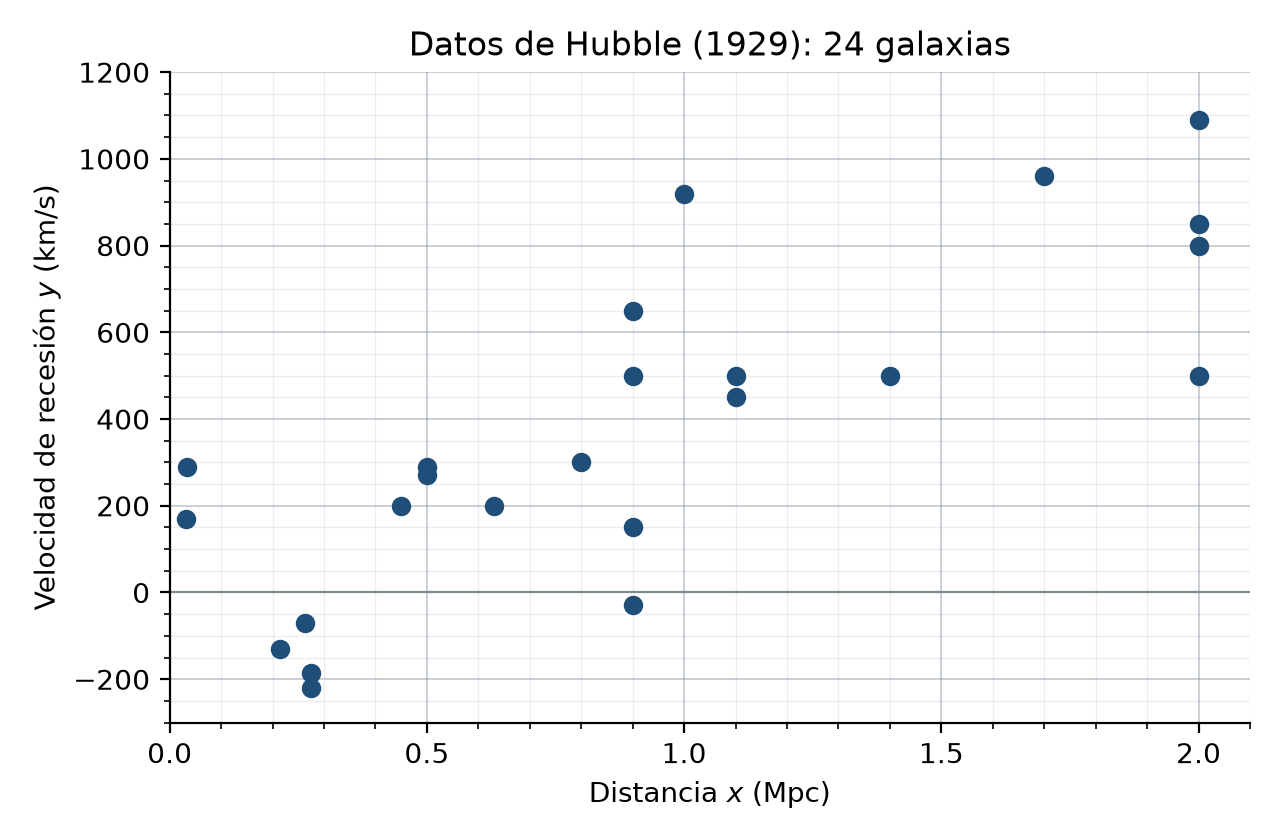
\includegraphics[width=\linewidth]{01_dispersion.png}
    \column{0.40\textwidth}
      \tarjeta[<2->]{Tendencia}{A 2 Mpc las velocidades van de 500 a 1090 km/s; bajo 0.5 Mpc, de $-220$ a 290 km/s.}
      \tarjeta[<3->]{Forma}{Sin curvatura clara: $y = ax + b$ es razonable.}
      \tarjeta[<4->]{Dispersión}{Grande: para una misma distancia hay velocidades muy distintas.}
  \end{columns}
  \note{Antes de calcular, miramos los datos. La nube sube y no se curva, así que el modelo lineal es una primera aproximación razonable. Ya se nota que la recta no pasará cerca de todos los puntos.}
\end{frame}

\begin{frame}{Cada recta saca una nota: su error $S(a,b)$}
  \framesubtitle{Construcción del modelo}
  \begin{columns}[T]
    \column{0.31\textwidth}\tarjeta{Predicción}{\[\hat y_i = a x_i + b\]}
    \column{0.31\textwidth}\tarjeta[<2->]{Residuo}{\[e_i = y_i - (a x_i + b)\]}
    \column{0.31\textwidth}\tarjeta[<3->]{Error cuadrático}{\[S(a,b) = \sum_{i=1}^{n} e_i^2\]}
  \end{columns}
  \vfill
  \uncover<4->{\textbf{\color{tinta}El cambio de papel:} los 24 pares $(x_i, y_i)$ son números fijos y las variables son $a$ y $b$. Cada punto del plano $(a,b)$ es una recta distinta, y buscamos la de menor error.}
  \vspace{0.6em}

  \uncover<3->{\small Se eleva al cuadrado para que los errores positivos y negativos no se cancelen y para que $S$ sea derivable.}
  \note{Si sumáramos los residuos sin elevarlos, una recta pésima podría dar suma cero. Al desarrollar, S es un polinomio de grado 2 en a y b: su gráfica es un paraboloide.}
\end{frame}

% =====================================================================
% 2. DESARROLLO ANALÍTICO
% =====================================================================
\begin{frame}{Derivadas parciales}
  \framesubtitle{Desarrollo analítico · a mano}
  \begin{align*}
    \uncover<2->{\frac{\partial S}{\partial a}} &\uncover<2->{= \sum_{i=1}^{n} 2(y_i - a x_i - b)\cdot(-x_i)} \uncover<3->{= \boxed{-2\sum_{i=1}^{n} x_i\,(y_i - a x_i - b)}} \\[0.6em]
    \uncover<4->{\frac{\partial S}{\partial b}} &\uncover<4->{= \sum_{i=1}^{n} 2(y_i - a x_i - b)\cdot(-1)} \uncover<5->{= \boxed{-2\sum_{i=1}^{n} (y_i - a x_i - b)}}
  \end{align*}
  \vfill
  \begin{columns}[T]
    \column{0.31\textwidth}\tarjeta{Regla de la cadena}{$(u^2)' = 2u\,u'$, con $u = y_i - a x_i - b$.}
    \column{0.31\textwidth}\tarjeta[<2->]{Respecto de $a$}{$b$ queda constante, así que $u' = -x_i$.}
    \column{0.31\textwidth}\tarjeta[<4->]{Respecto de $b$}{$a$ queda constante, así que $u' = -1$.}
  \end{columns}
  \note{La derivada respecto de a mide cuánto cambia el error si movemos solo la pendiente; respecto de b, si movemos solo el intercepto. Geométricamente son las pendientes de la superficie en cada dirección.}
\end{frame}

\begin{frame}{$\nabla S = \mathbf{0}$ da un sistema lineal $2\times 2$}
  \framesubtitle{Desarrollo analítico · a mano}
  \begin{columns}[c]
    \column{0.6\textwidth}
      {\scriptsize\bfseries\color{acento}ECUACIONES NORMALES}
      \begin{align*}
        a\sum x_i^2 + b\sum x_i &= \sum x_i y_i \\
        a\sum x_i + n\,b &= \sum y_i
      \end{align*}
      \uncover<3->{%
      {\scriptsize\bfseries\color{acento}CON LOS DATOS DE HUBBLE}
      \begin{align*}
        29.517795\,a + 21.873\,b &= 12\,513.695 \\
        21.873\,a + 24\,b &= 8\,955
      \end{align*}}
    \column{0.34\textwidth}
      \tarjeta[<2->]{Las cinco sumas}{%
        $n = 24$\\[0.3em]
        $\sum x_i = 21.873$\\[0.3em]
        $\sum y_i = 8\,955$\\[0.3em]
        $\sum x_i^2 = 29.517795$\\[0.3em]
        $\sum x_i y_i = 12\,513.695$}
  \end{columns}
  \note{Igualamos las dos derivadas a cero, dividimos entre -2 y separamos las sumas. Lo único que hace falta de los datos son cinco sumas, que verificamos con calculadora.}
\end{frame}

\begin{frame}{Solución del sistema}
  \framesubtitle{Desarrollo analítico · a mano}
  \[
    a^* = \frac{n\sum x_i y_i - \sum x_i \sum y_i}{n\sum x_i^2 - \left(\sum x_i\right)^2} = \frac{104\,455.965}{229.998951},
    \qquad b^* = \bar y - a^*\bar x
  \]
  \vfill
  \begin{columns}[T]
    \column{0.31\textwidth}\tarjeta[<2->]{Pendiente $a^*$}{\grande{454.16}\\[0.3em]km/s por Mpc: la constante de Hubble estimada.}
    \column{0.31\textwidth}\tarjeta[<3->]{Intercepto $b^*$}{\grande{$-$40.78}\\[0.3em]km/s: cerca de 0, como pide la física.}
    \column{0.31\textwidth}\tarjeta[<4->]{Error mínimo}{\grande{1\,193\,442}\\[0.3em](km/s)$^2$: nunca es 0, ninguna recta toca los 24 puntos.}
  \end{columns}
  \note{a* sale por Cramer o sustitución. Ojo con el redondeo: con a* = 454.16 ya redondeado, b sale -40.79; con a* sin redondear sale -40.78. Ambas son correctas dentro del redondeo.}
\end{frame}

\begin{frame}{El Hessiano demuestra que es un mínimo}
  \framesubtitle{Desarrollo analítico · a mano}
  \begin{columns}[c]
    \column{0.52\textwidth}
      \begin{align*}
        H &= \begin{pmatrix} S_{aa} & S_{ab} \\ S_{ba} & S_{bb} \end{pmatrix}
           = \begin{pmatrix} 2\sum x_i^2 & 2\sum x_i \\ 2\sum x_i & 2n \end{pmatrix} \\[0.4em]
          &\uncover<2->{= \begin{pmatrix} 59.036 & 43.746 \\ 43.746 & 48 \end{pmatrix}}
      \end{align*}
      \uncover<2->{Es \textbf{\color{tinta}constante}: no depende de $a$ ni de $b$, solo de los $x_i$.}
    \column{0.44\textwidth}
      \tarjeta[<3->]{Determinante}{$\det H = (59.036)(48) - 43.746^2$\\$\phantom{\det H}\approx 920 > 0$}
      \tarjeta[<4->]{Curvatura}{$S_{aa} = 59.036 > 0 \;\Rightarrow\;$ mínimo}
      \tarjeta[<5->]{Global, no solo local}{$\det H = 4n\sum (x_i - \bar x)^2 > 0$ si hay dos $x$ distintos. $S$ es un paraboloide convexo.}
  \end{columns}
  \note{Criterio de la segunda derivada: D > 0 y S_aa > 0 implica mínimo. Los valores propios son 9.43 y 97.61, ambos positivos. Como S es de grado 2, su Taylor alrededor del óptimo es exacto y el término lineal se anula: cualquier otra recta tiene más error, así que el mínimo es global.}
\end{frame}

% =====================================================================
% 3. GEOMETRÍA
% =====================================================================
\begin{frame}{La superficie de error es un valle con un solo fondo}
  \framesubtitle{Interpretación geométrica}
  \begin{columns}[c]
    \column{0.52\textwidth}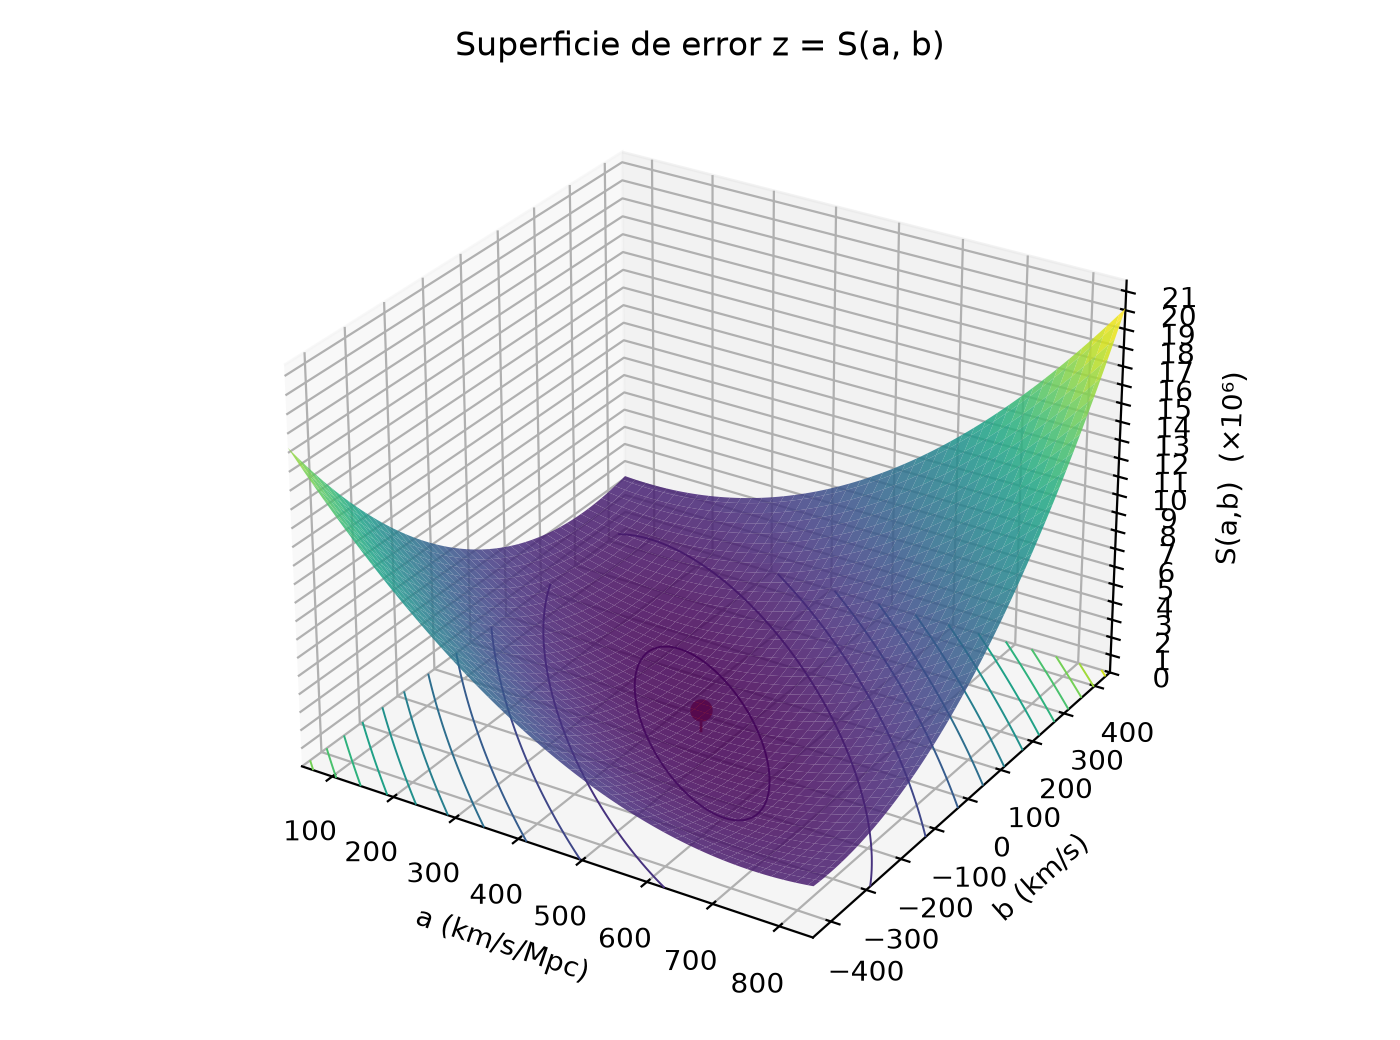
\includegraphics[width=\linewidth]{03_superficie.png}
    \column{0.44\textwidth}
      \tarjeta[<2->]{Forma}{Paraboloide abierto hacia arriba, alargado como un valle.}
      \tarjeta[<3->]{Mínimo}{Un único punto más bajo en $(a^*, b^*) \approx (454.2,\,-40.8)$.}
      \tarjeta[<4->]{Altura del fondo}{$S_{\min} \approx 1.19\times 10^6$, no cero: siempre queda un error.}
  \end{columns}
  \note{Cada punto del piso es una recta y la altura es su error. Lo que el Hessiano dijo con números, la superficie lo muestra: curvatura positiva en todas partes y un solo fondo.}
\end{frame}

\begin{frame}{Trazas y secciones: parábolas que se desplazan}
  \framesubtitle{Interpretación geométrica}
  \centering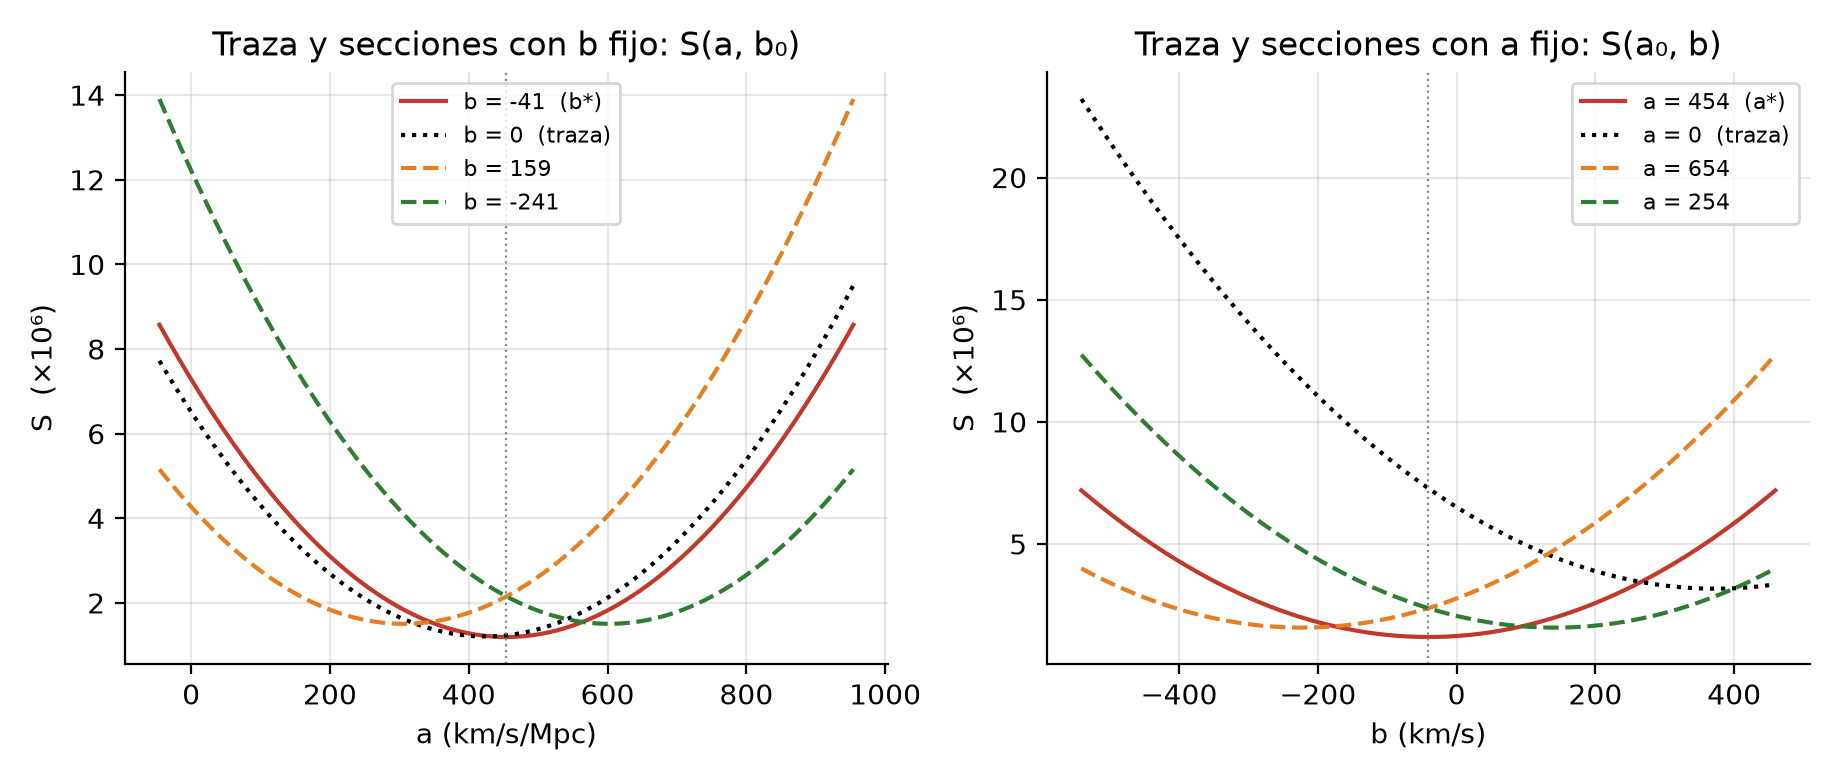
\includegraphics[height=0.47\textheight]{04_trazas.png}
  \vfill
  \begin{columns}[T]
    \column{0.31\textwidth}\tarjeta[<2->]{Abren hacia arriba}{Todas con la misma abertura: el Hessiano constante visto en 1D.}
    \column{0.31\textwidth}\tarjeta[<3->]{El vértice se mueve}{Si $b$ sube, el mejor $a$ baja: $S_{ab} = 2\sum x_i \neq 0$, se compensan.}
    \column{0.31\textwidth}\tarjeta[<4->]{Traza $b = 0$}{Recta por el origen, la ley de Hubble pura: mínimo en $a \approx 423.9$.}
  \end{columns}
  \note{Fijar b deja una parábola en a con segunda derivada 2 suma x^2 = 59.04; fijar a deja una parábola en b con segunda derivada 2n = 48. La traza a = 0 es la recta horizontal y = ybarra = 373.1, el modelo con el que se compara R^2.}
\end{frame}

\begin{frame}{Curvas de nivel: elipses alrededor de $(a^*, b^*)$}
  \framesubtitle{Interpretación geométrica}
  \begin{columns}[c]
    \column{0.46\textwidth}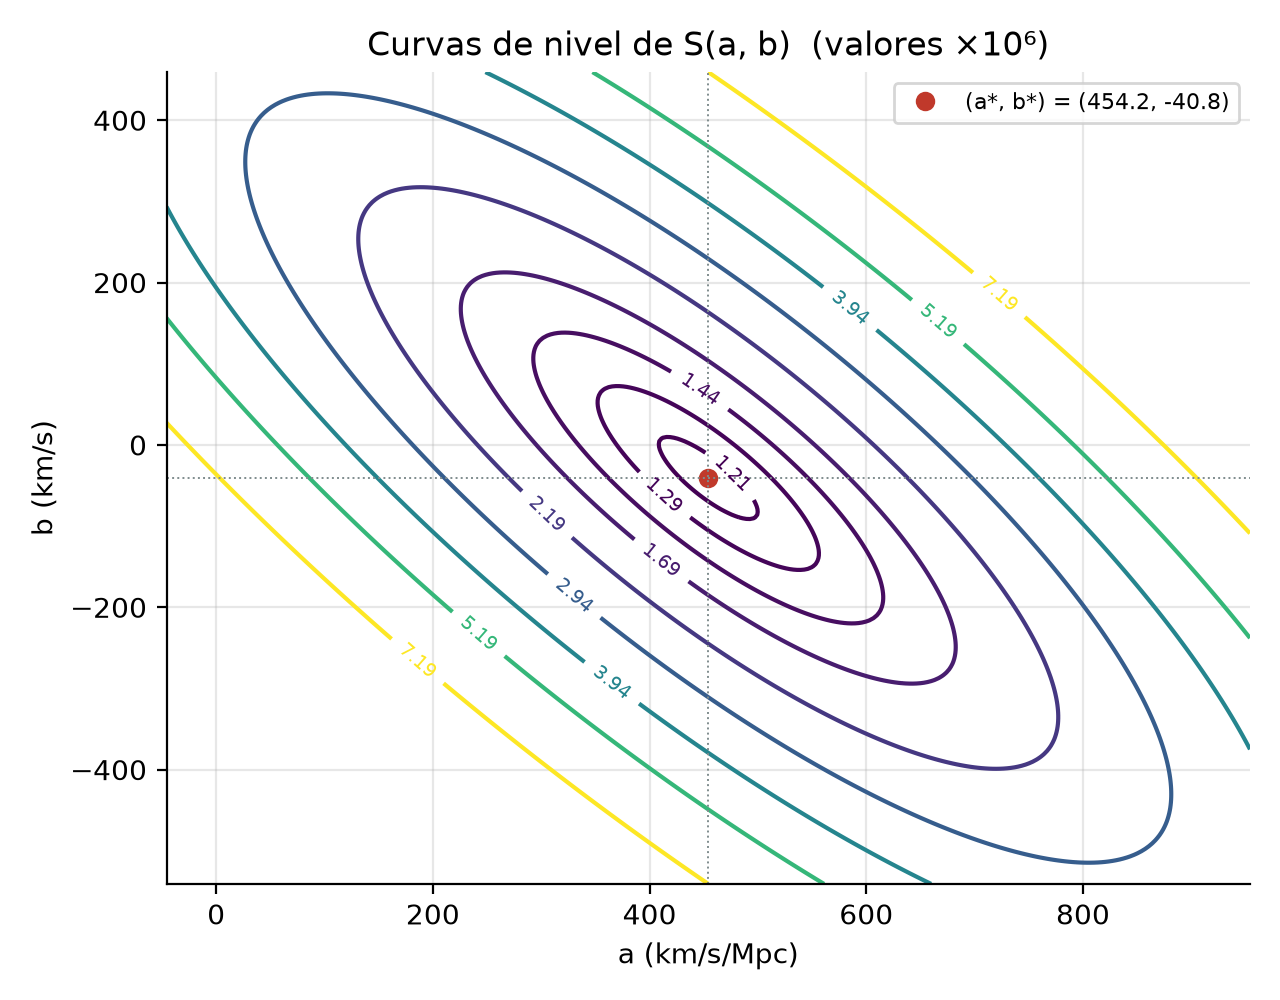
\includegraphics[width=\linewidth]{05_curvas_nivel.png}
    \column{0.25\textwidth}
      \tarjeta[<2->]{Concéntricas}{Cada elipse reúne rectas con el mismo error; el mínimo es el punto que todas encierran.}
      \tarjeta[<4->]{Alargadas}{Ejes en razón $\sqrt{\lambda_2/\lambda_1}\approx 3.2$: una dirección está peor determinada.}
    \column{0.25\textwidth}
      \tarjeta[<3->]{Inclinadas}{Se puede subir $a$ y bajar $b$ sin que el error cambie mucho.}
      \tarjeta[<5->]{Gradiente}{Perpendicular a las curvas, hacia afuera, y nulo en el centro: $\nabla S = \mathbf{0}$.}
  \end{columns}
  \note{Es el mapa visto desde arriba. Los valores crecen hacia afuera: alejarse del centro en cualquier dirección aumenta el error. lambda1 = 9.43 y lambda2 = 97.61 son los valores propios del Hessiano.}
\end{frame}

% =====================================================================
% 4. VERIFICACIÓN
% =====================================================================
\begin{frame}{Cada función del código es una fórmula del desarrollo}
  \framesubtitle{Verificación computacional}
  \small
  \begin{tabularx}{\textwidth}{l >{\raggedright\arraybackslash}X l}
    \toprule
    \textbf{Función} & \textbf{Fórmula que implementa} & \textbf{Resultado} \\
    \midrule
    \texttt{sumas()} & $n,\ \sum x,\ \sum y,\ \sum x^2,\ \sum xy$ & Las cinco sumas \\
    \texttt{ajustar()} & Regla de Cramer sobre $\nabla S = \mathbf{0}$ & $a^* = 454.158$, $b^* = -40.784$ \\
    \texttt{error\_cuadratico()} & $S(a,b) = \sum (y_i - a x_i - b)^2$ & $S_{\min} = 1\,193\,442.37$ \\
    \texttt{gradiente()} & $\left(-2\sum x_i e_i,\ -2\sum e_i\right)$ & $\approx (1.8\cdot10^{-11},\ 1.9\cdot10^{-11})$ \\
    \texttt{hessiano()} & $\left(\begin{smallmatrix} 2\sum x^2 & 2\sum x \\ 2\sum x & 2n\end{smallmatrix}\right)$ & $\det \approx 920$; $\lambda = 9.43,\ 97.61$ \\
    \texttt{hessiano\_numerico()} & Diferencias finitas de $S$ (\texttt{verificacion.py}) & Coincide con $H$ a $10^{-4}$ \\
    \bottomrule
  \end{tabularx}
  \vfill
  {\footnotesize Sin funciones de regresión de librería en el método propio (\texttt{codigo/regresion.py}). Pseudocódigo y diagrama de flujo en \texttt{docs/pseudocodigo.md}.}
  \note{Flujo: cargar datos, calcular sumas, verificar que el determinante no sea cero, resolver a y b, calcular S, gradiente y Hessiano, y graficar. El gradiente en el óptimo es del orden de 1e-11 por el redondeo de punto flotante.}
\end{frame}

\begin{frame}{A mano, código propio y librerías dan lo mismo}
  \framesubtitle{Comparación entre métodos}
  \footnotesize
  % TODO: reemplazar la columna "A mano" por los valores obtenidos en el desarrollo en papel.
  \begin{tabularx}{\textwidth}{l *{5}{>{\raggedleft\arraybackslash}X}}
    \toprule
    \textbf{Parámetro} & \textbf{A mano} & \textbf{Código propio} & \textbf{\texttt{numpy.polyfit}} & \textbf{\texttt{scipy linregress}} & \textbf{Dif. máxima} \\
    \midrule
    $a$ & 454.16 & 454.158441 & 454.158441 & 454.158441 & $1.6\cdot10^{-3}$ \\
    $b$ & $-40.79$ & $-40.783649$ & $-40.783649$ & $-40.783649$ & $6.4\cdot10^{-3}$ \\
    $S_{\min}$ & 1\,193\,442.367 & 1\,193\,442.366 & 1\,193\,442.366 & 1\,193\,442.366 & $6.1\cdot10^{-4}$ \\
    \bottomrule
  \end{tabularx}
  \vfill
  \begin{columns}[T]
    \column{0.31\textwidth}\tarjeta[<2->]{Código vs librerías}{Difieren en $10^{-13}$: redondeo de máquina. Las librerías resuelven lo mismo con otro algoritmo.}
    \column{0.31\textwidth}\tarjeta[<3->]{A mano vs código}{La diferencia viene del redondeo a dos decimales, no del método.}
    \column{0.31\textwidth}\tarjeta[<4->]{$S$ casi no cambia}{En el mínimo $\nabla S = \mathbf{0}$: un cambio pequeño en $(a,b)$ mueve $S$ solo en segundo orden.}
  \end{columns}
  \note{IMPORTANTE: la columna A mano debe llevar los valores del desarrollo en papel. La librería se usó solo como verificación, como pide el enunciado.}
\end{frame}

% =====================================================================
% 5. ANÁLISIS
% =====================================================================
\begin{frame}{$y = 454.2\,x - 40.8$ sigue la tendencia, no cada galaxia}
  \framesubtitle{Análisis de la recta de ajuste}
  \begin{columns}[c]
    \column{0.56\textwidth}
      % Mismos datos y rectas que graficos/02_recta_ajuste.png, dibujados por pasos
      \begin{tikzpicture}[x=3.25cm,y=0.0034cm,font=\tiny]
        \fill[white] (-0.02,-310) rectangle (2.12,1210);
        \foreach \v in {-200,0,...,1200} {\draw[cuerpo!12] (0,\v) -- (2.1,\v); \node[left] at (0,\v) {\v};}
        \foreach \u in {0,0.5,1,1.5,2} {\draw[cuerpo!12] (\u,-300) -- (\u,1200); \node[below] at (\u,-300) {\u};}
        \draw[cuerpo!60] (0,-300) rectangle (2.1,1200);
        \node[below=9pt] at (1.05,-300) {Distancia $x$ (Mpc)};
        \node[rotate=90,above=14pt] at (0,450) {Velocidad $y$ (km/s)};
        \begin{scope}
          \clip (0,-300) rectangle (2.1,1200);
          \only<2->{%
            \draw[cuerpo!55,dashed,thick] (0,-191) -- (2.1,{704*2.1-191});
            \draw[blue!60!black,dashed,thick] (0,159) -- (2.1,{204*2.1+159});
            \draw[green!45!black,dashed,thick] (0,209) -- (2.1,{454*2.1+209});}
          \only<3->{\draw[acento,line width=1.6pt] (0,-40.78) -- (2.1,{454.16*2.1-40.78});}
        \end{scope}
        \foreach \x/\y in {0.032/170,0.034/290,0.214/-130,0.263/-70,0.275/-185,0.275/-220,0.45/200,0.5/290,0.5/270,0.63/200,0.8/300,0.9/-30,0.9/650,0.9/150,0.9/500,1.0/920,1.1/450,1.1/500,1.4/500,1.7/960,2.0/500,2.0/850,2.0/800,2.0/1090}
          \fill[tinta] (\x,\y) circle (1.6pt);
        \only<4->{%
          \foreach \x/\y/\n/\p in {1.0/920/NGC 1068/right,0.9/-30/NGC 3031/below right,2.0/500/NGC 4382/below left}
            {\draw[acento,thick] (\x,\y) circle (4pt); \node[\p,text=acento,font=\tiny\bfseries] at (\x,\y) {\n};}}
        \only<5->{%
          \draw[naranja,thick,densely dotted,rounded corners] (1.95,430) rectangle (2.06,1150);
          \draw[naranja,thick,densely dotted,rounded corners] (-0.02,120) rectangle (0.09,340);}
        \tikzset{ley/.style={anchor=west,fill=white,fill opacity=0.9,text opacity=1,inner sep=1.5pt}}
        \node<2->[ley] at (0.03,1150) {{\color{cuerpo!55}- - -} $a{=}704,\ b{=}{-191}$: $S = 1.94\cdot10^6$};
        \node<2->[ley] at (0.03,1075) {{\color{blue!60!black}- - -} $a{=}204,\ b{=}159$: $S = 1.81\cdot10^6$};
        \node<2->[ley] at (0.03,1000) {{\color{green!45!black}- - -} $a{=}454,\ b{=}209$: $S = 2.60\cdot10^6$};
        \node<3->[ley] at (0.03,925) {{\color{acento}\textbf{---}} óptima: $S = 1.19\cdot10^6$};
      \end{tikzpicture}
    \column{0.40\textwidth}
      \tarjeta[<2->]{Otras rectas}{Las tres punteadas tienen un error 1.5 a 2.2 veces mayor: cada una está en una curva de nivel más externa.}
      \tarjeta[<4->]{Más desviadas}{NGC 1068 ($+507$ km/s), NGC 3031 ($-398$) y NGC 4382 ($-368$).}
      \tarjeta[<5->]{Posibles influyentes}{Las galaxias a 2 Mpc y las Nubes de Magallanes, en los extremos de $x$: tienen palanca.}
  \end{columns}
  \note{La recta atraviesa la nube por el centro. Cambiar la pendiente o desplazar la recta siempre aumenta S: eso significa que sea el mínimo.}
\end{frame}

\begin{frame}{Residuos $e_i = y_i - (a^* x_i + b^*)$}
  \framesubtitle{Análisis de los residuos}
  \begin{columns}[c]
    \column{0.48\textwidth}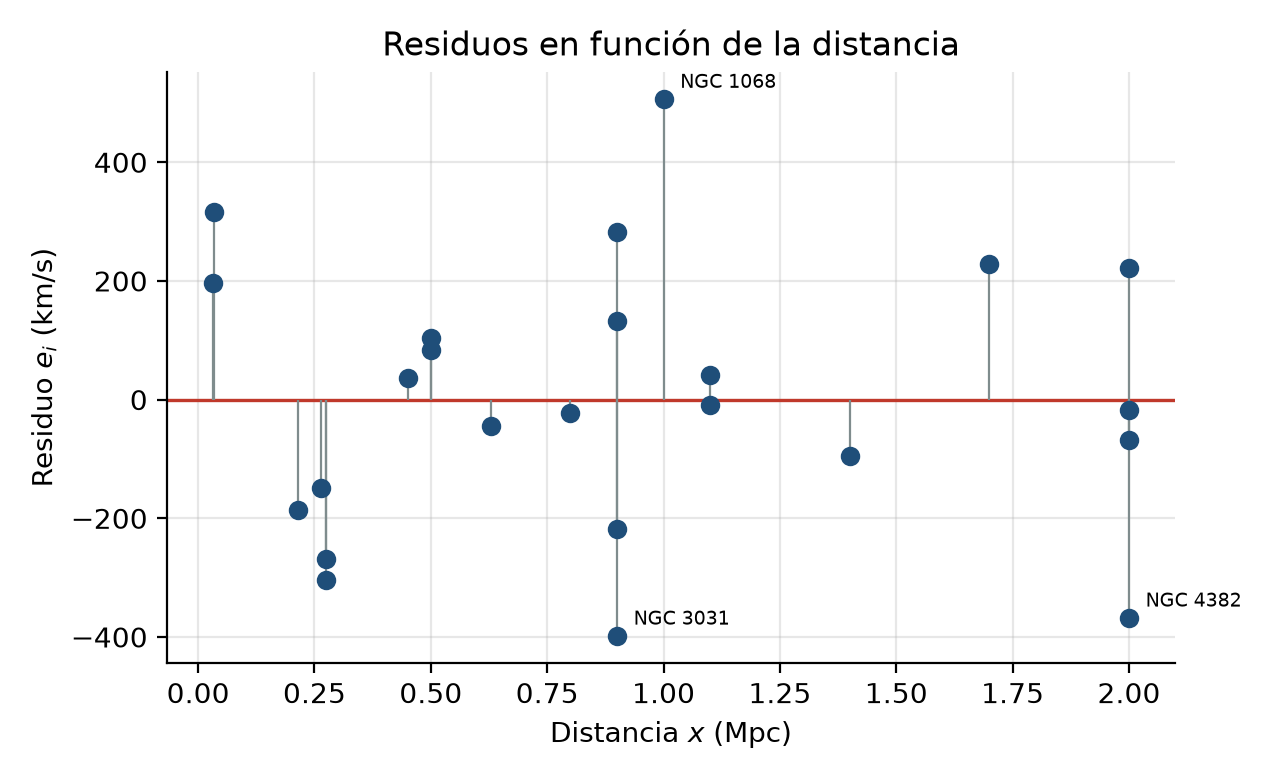
\includegraphics[width=\linewidth]{06_residuos.png}
    \column{0.48\textwidth}\uncover<2->{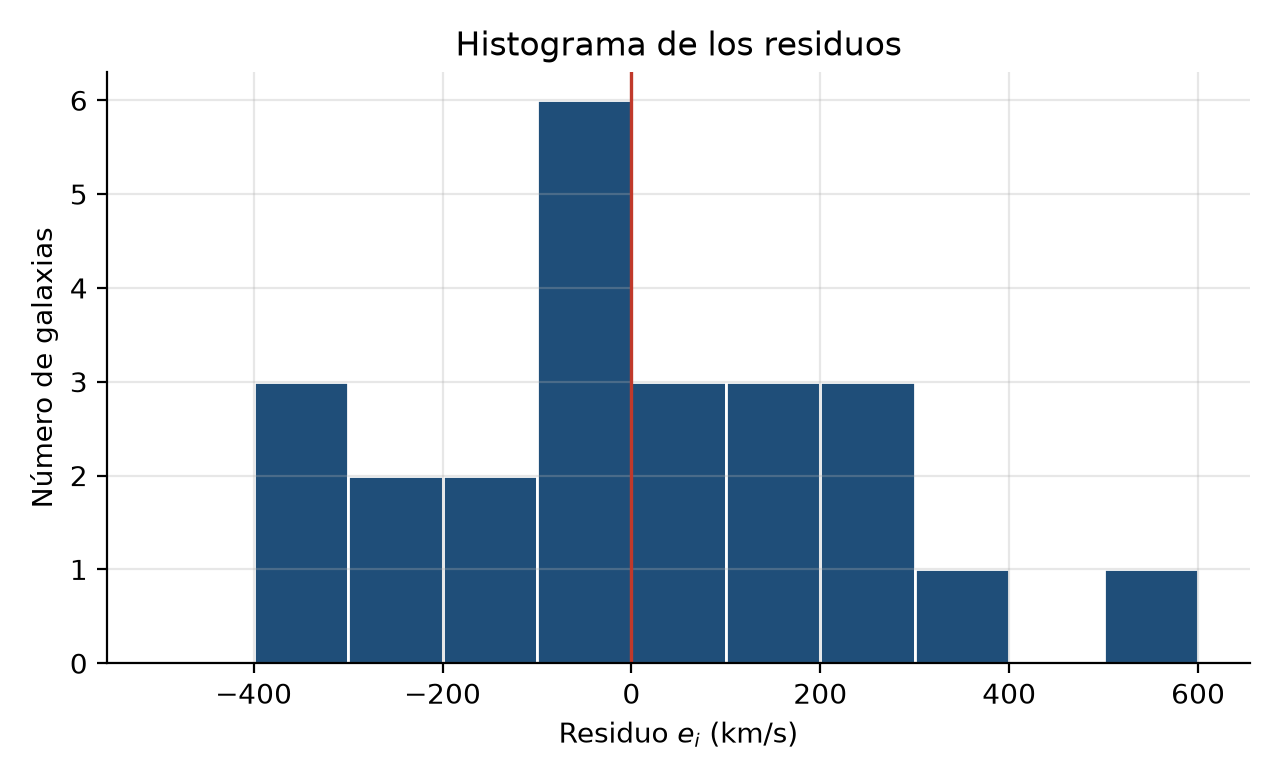
\includegraphics[width=\linewidth]{07_histograma_residuos.png}}
  \end{columns}
  \vfill
  \uncover<3->{\textbf{\color{tinta}En una frase:} centrados en cero y sin curva global, pero con una desviación sistemática en las galaxias más cercanas.}
  \note{A la izquierda, cada residuo contra su distancia; a la derecha, su distribución. En la siguiente diapositiva respondemos las preguntas del enunciado una por una.}
\end{frame}

\begin{frame}{Qué dicen los residuos}
  \framesubtitle{Análisis de los residuos}
  \begin{columns}[T]
    \column{0.48\textwidth}
      \tarjeta{¿Centrados en cero?}{Sí: 11 positivos, 13 negativos y media 0. No es suerte: $\partial S/\partial b = 0$ obliga a que $\sum e_i = 0$.}
      \tarjeta[<3->]{¿Atípicos?}{NGC 1068 ($+507$), NGC 3031 ($-398$), NGC 4382 ($-368$): unas dos veces el RMSE. Grandes, pero no hay razón para descartarlos.}
    \column{0.48\textwidth}
      \tarjeta[<2->]{¿Tendencia o patrón?}{No hay U ni rampa global, lo que apoya el modelo lineal. Además $\sum x_i e_i = 0$ por $\partial S/\partial a = 0$.}
      \tarjeta[<4->]{¿Desviación sistemática?}{Sí, cerca: entre 0.2 y 0.3 Mpc todos son negativos y en las Nubes de Magallanes positivos. Ahí domina el movimiento propio por la gravedad local.}
  \end{columns}
  \note{La dispersión es grande en todo el rango (entre -400 y +500 km/s) y no crece claramente con x. Andrómeda (NGC 224) de hecho se acerca a nosotros. Conclusión: compatible con un modelo lineal para la tendencia, con dos reservas.}
\end{frame}

\begin{frame}{RMSE y $R^2$, leídos con los datos de Hubble}
  \framesubtitle{Calidad del modelo}
  \begin{columns}[T]
    \column{0.48\textwidth}\tarjeta{$\mathrm{RMSE} = \sqrt{S/n}$}{\grande{223 km/s}\\[0.4em]Error típico al predecir la velocidad de una galaxia por su distancia. Es grande frente a la velocidad media de 373 km/s.}
    \column{0.48\textwidth}\tarjeta[<2->]{$R^2 = 1 - S\,/\sum (y_i - \bar y)^2$}{\grande{0.62}\\[0.4em]La distancia explica cerca del 62\,\% de la variación de las velocidades; el 38\,\% restante son movimientos propios y errores de distancia.}
  \end{columns}
  \vfill
  \uncover<3->{\textbf{\color{tinta}Para el propósito de Hubble basta:} probar que la relación existe y estimar la pendiente. Para predecir una galaxia individual, no.}
  \note{R^2 compara la recta con el modelo sin pendiente y = ybarra, que es la traza a = 0. r = 0.79. Un R^2 mayor no habría corregido la pendiente: el problema estaba en las distancias medidas.}
\end{frame}

\begin{frame}{Quitar una sola galaxia mueve la pendiente un 11\,\%}
  \framesubtitle{Análisis adicional · opción B}
  \centering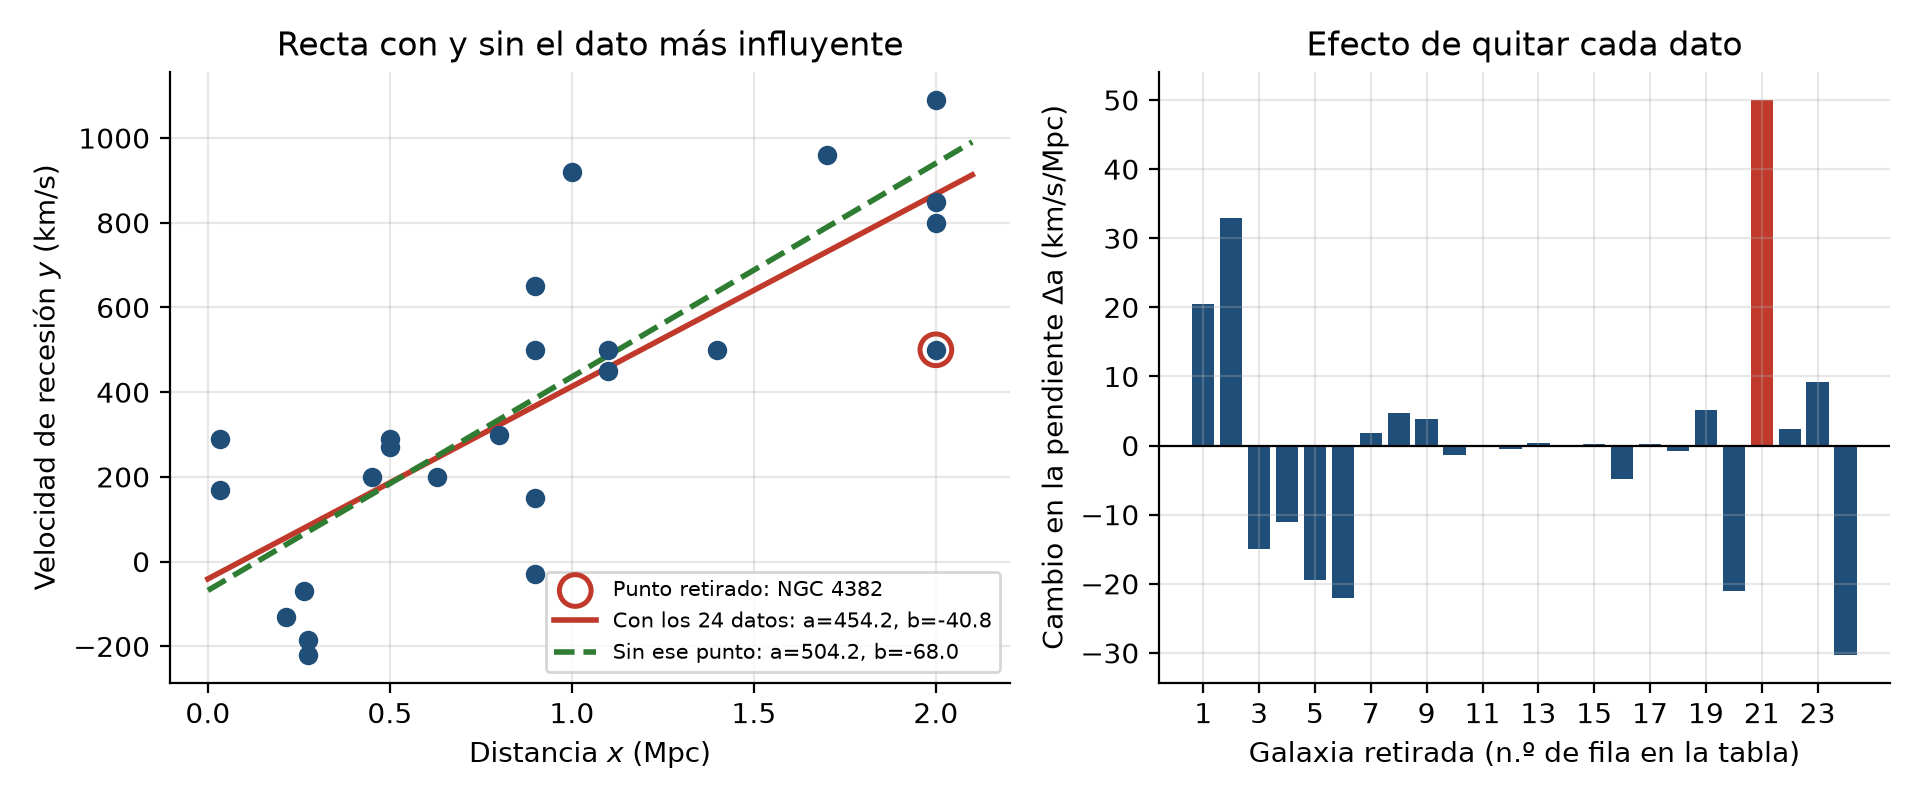
\includegraphics[height=0.45\textheight]{08_influencia.png}
  \vfill
  \begin{columns}[T]
    \column{0.31\textwidth}\tarjeta[<2->]{NGC 4382}{Sin ella, $a$ pasa de 454 a 504 km/s/Mpc. Está en el extremo ($x = 2$ Mpc) y su velocidad es baja.}
    \column{0.31\textwidth}\tarjeta[<3->]{Palanca}{Los puntos más influyentes están lejos de $\bar x$, en los extremos de la distancia.}
    \column{0.31\textwidth}\tarjeta[<4->]{NGC 1068}{El mayor residuo, pero $\Delta a = -4.9$. Está cerca de $\bar x$: mueve $b$, no $a$.}
  \end{columns}
  \note{Se quita cada galaxia, se recalcula con las 23 restantes y se repite para las 24. La pendiente queda siempre entre 424 y 504: la conclusión cualitativa no depende de ningún dato, pero el valor exacto sí es sensible a unos pocos.}
\end{frame}

% =====================================================================
% 6. CIERRE
% =====================================================================
{\begin{oscura}
\begin{frame}{La respuesta a la pregunta central}
  \framesubtitle{Conclusiones}
  \begin{columns}[T]
    \column{0.48\textwidth}
      \tarjeta{Analítica}{$\nabla S = \mathbf{0}$ convierte ``la mejor recta'' en un sistema $2\times2$ con solución única: $a^*\approx 454.2$ km/s/Mpc, $b^* \approx -40.8$ km/s. El Hessiano constante y definido positivo garantiza un mínimo global.}
      \tarjeta[<3->]{Computacional}{El método propio coincide con numpy y scipy hasta $10^{-13}$ y con el cálculo a mano hasta el redondeo. El computador verifica; no reemplaza.}
    \column{0.48\textwidth}
      \tarjeta[<2->]{Geométrica}{La superficie es un valle con un solo fondo, las secciones son parábolas y las curvas de nivel elipses centradas en $(a^*, b^*)$. Su inclinación muestra que $a$ y $b$ se compensan.}
      \tarjeta[<4->]{Sobre los datos}{La recta capta la tendencia ($R^2\approx 0.62$), no cada galaxia; falla de forma sistemática en las más cercanas, y un solo dato mueve la pendiente hasta un 11\,\%.}
  \end{columns}
  \note{Volver a la pregunta central: el Cálculo Multivariable permite determinar el modelo (gradiente cero), garantizar que es el mejor (Hessiano) y entenderlo (superficie, trazas, curvas de nivel); residuos, R^2 e influencia dicen hasta dónde confiar en él.}
\end{frame}
\end{oscura}}

{\begin{acento}
\begin{frame}{Un ajuste perfecto no corrige datos sesgados}
  \framesubtitle{Reflexión crítica}
  Las distancias de 1929 estaban subestimadas. Con nuestra pendiente, la edad del universo, $1/H_0$, sería unos 2\,150 millones de años: menos que la edad de la Tierra.
  \vspace{0.6em}
  \begin{columns}[T]
    \column{0.48\textwidth}\tarjeta[<2->]{Hubble 1929}{\grande{454}\\[0.3em]km/s por Mpc}
    \column{0.48\textwidth}\tarjeta[<3->]{Valor actual}{\grande{$\approx$ 70}\\[0.3em]km/s por Mpc: 6.5 veces menor}
  \end{columns}
  \vfill
  \footnotesize
  \uncover<4->{\begin{columns}[T]
    \column{0.23\textwidth} El método supone error solo en $y$; aquí $x$ también lo tiene.
    \column{0.23\textwidth} Al elevar al cuadrado, los extremos pesan mucho.
    \column{0.23\textwidth} 24 galaxias hasta 2 Mpc: no se puede extrapolar lejos.
    \column{0.23\textwidth} $b \neq 0$; sin intercepto, $y = ax$ daría $a \approx 424$.
  \end{columns}}
  \note{Mínimos cuadrados encuentra la mejor recta para los datos que se le dan; si las mediciones tienen un error sistemático, la recta lo hereda. La tendencia de Hubble era correcta; el valor de la pendiente, no.}
\end{frame}
\end{acento}}

{\begin{oscura}
\begin{frame}[plain]
  \vfill
  {\scriptsize\bfseries\color{naranja}GRACIAS}\par\vspace{0.6em}
  {\fontsize{40}{44}\selectfont\bfseries ¿Preguntas?\par}\vspace{1em}
  $\nabla S(a^*, b^*) = \mathbf{0} \quad\cdot\quad \det H \approx 920 > 0 \quad\cdot\quad a^* \approx 454.16 \quad\cdot\quad b^* \approx -40.78$
  \vfill
  {\scriptsize Material: guía del proyecto, código en \texttt{codigo/} y desarrollo a mano en \texttt{analisis\_manual/}.}
  \note{Preguntas probables: por qué se elevan al cuadrado los residuos, por qué el Hessiano no depende de a ni de b, qué significa que las curvas de nivel estén inclinadas, por qué la suma de residuos es cero, por qué NGC 4382 influye más que NGC 1068.}
\end{frame}
\end{oscura}}

\end{document}
